\documentclass[conference]{IEEEtran}
\usepackage[utf8]{inputenc}
\usepackage[spanish]{babel}
\usepackage{amsmath,amssymb,amsfonts}
\usepackage{graphicx}
\usepackage{cite}
\usepackage{hyperref}
\usepackage{algorithm}
\usepackage{algorithmic}

\begin{document}

\title{Eficiencia Espectral de la División del Trabajo Humano: Comparación de Particiones Observadas con Bisecciones de Fiedler}

\author{\IEEEauthorblockN{Thomas Chísica}
\IEEEauthorblockA{Universidad del Rosario\\
Teoría de Grafos 2026-I\\
Profesor: Daniel Alfonso Bojacá Torres}}

\maketitle

% ============================================================================
% SECCIÓN 1: INTRODUCCIÓN
% ============================================================================
\section{Introducción}

La coordinación entre agentes que no pueden comunicarse explícitamente representa un problema fundamental en sistemas multi-agente y ciencias cognitivas. Cuando múltiples individuos deben colaborar para completar una tarea compartida sin posibilidad de negociación directa, emergen patrones de división del trabajo que optimizan el rendimiento grupal de manera auto-organizada \cite{andrade2021}. Este fenómeno puede modelarse rigurosamente mediante teoría algebraica de grafos, donde el espacio de interacción constituye un grafo y las divisiones emergentes corresponden a particiones cuya calidad puede cuantificarse espectralmente.

En el experimento ``Seeking the Unicorn'' desarrollado por Andrade-Lotero y Goldstone \cite{andrade2021}, parejas de participantes humanos buscan un objetivo oculto en un tablero compartido de $8 \times 8$ celdas. Sin comunicación explícita, las díadas desarrollan divisiones espaciales del trabajo---típicamente izquierda-derecha o arriba-abajo---que minimizan la redundancia y maximizan la cobertura conjunta. La pregunta central de este proyecto es: \textbf{¿son estas divisiones espectralmente eficientes?}

Este proyecto no busca validar la Desigualdad de Cheeger (un resultado teórico establecido \cite{chung1997}), sino utilizar el \textbf{vector de Fiedler} como benchmark de optimalidad. Se comparará la conductancia de las particiones empíricas generadas por los humanos $h(S_{\text{obs}})$ contra la conductancia de la bisección espectral teórica $h(S_{\text{Fiedler}})$ y la cota inferior $\lambda_2/2$. Nuestra hipótesis es que la coordinación humana implícita converge a soluciones cercanas al óptimo espectral.

La relevancia de este trabajo radica en su conexión con la Teoría Algebraica de Grafos \cite{chung1997, fiedler1973} y con la bibliografía del curso sobre métodos graph-teóricos en redes multi-agente \cite{mesbahi2010}.

% ============================================================================
% SECCIÓN 2: DESCRIPCIÓN DEL PROBLEMA
% ============================================================================
\section{Descripción del Problema}

\subsection{Contexto Experimental}

El dataset ``Self-Organized Division of Cognitive Labor'' (SODCL) \cite{andrade2021} contiene datos de comportamiento de 45 díadas a lo largo de 60 rondas cada una. En cada ronda, cada jugador selecciona hasta 32 celdas de un tablero de $8 \times 8$ para ``cubrir''. Las celdas cubiertas por ambos jugadores representan redundancia. A lo largo del experimento, las díadas desarrollan divisiones espaciales emergentes sin comunicación explícita.

Un análisis exploratorio preliminar revela patrones claros: la díada 435-261 exhibe una divergencia izquierda-derecha del 93.07\%, donde el Jugador 1 acumula 887 visitas en columnas 5-8 versus 43 en columnas 1-4, mientras el Jugador 2 muestra el patrón inverso (889 vs. 21).

\subsection{Formulación Graph-Teórica}

\textbf{Definición 1 (Grafo del Tablero).} Sea $G = (V, E)$ donde $V = \{(i,j) : 1 \leq i,j \leq 8\}$ representa las 64 celdas y $E$ conecta celdas adyacentes bajo 8-conectividad. Entonces $|V| = 64$ y $|E| = 210$.

\textbf{Definición 2 (Matriz Laplaciana).} Para el grafo $G$ con matriz de adyacencia $A$ y matriz de grados $D = \text{diag}(d_1, \ldots, d_n)$, la matriz Laplaciana es $L = D - A$. Los eigenvalores de $L$ satisfacen $0 = \lambda_1 \leq \lambda_2 \leq \cdots \leq \lambda_n$.

\textbf{Definición 3 (Conectividad Algebraica).} El segundo eigenvalor más pequeño $\lambda_2$ se denomina \textit{valor de Fiedler} o conectividad algebraica. El eigenvector asociado $\mathbf{v}_2$ es el \textit{vector de Fiedler}.

\textbf{Definición 4 (Conductancia de una Partición).} Para una partición $(S, \bar{S})$ de $V$, la conductancia se define como:
\begin{equation}
h(S) = \frac{|\{(u,v) \in E : u \in S, v \in \bar{S}\}|}{\min(\text{vol}(S), \text{vol}(\bar{S}))}
\end{equation}
donde $\text{vol}(S) = \sum_{v \in S} d_v$ es el volumen de $S$.

\textbf{Teorema (Desigualdad de Cheeger \cite{chung1997}).} Para cualquier grafo $G$:
\begin{equation}
\frac{\lambda_2}{2} \leq h(G) \leq \sqrt{2\lambda_2}
\end{equation}
donde $h(G) = \min_S h(S)$ es la constante de Cheeger (isoperimétrica) del grafo.

% ============================================================================
% SECCIÓN: DEGENERACIÓN DEL EIGENESPACIO DE FIEDLER
% ============================================================================
\subsection{Degeneración del Eigenespacio de Fiedler en la Grilla King}

El grafo del tablero $G = (V, E)$ con 8-conectividad corresponde al \textit{grafo king} $K(8,8)$, isomorfo al producto fuerte $P_8 \boxtimes P_8$ de dos caminos de longitud 8. Este grafo posee $|V| = 64$ vértices y $|E| = 210$ aristas, con distribución de grados: 4 vértices de esquina (grado 3), 24 vértices de borde (grado 5) y 36 vértices interiores (grado 8), verificándose $\sum_{v} d_v = 4(3) + 24(5) + 36(8) = 420 = 2|E|$.

\subsubsection{Simetría $D_4$ y Multiplicidad de $\lambda_2$}

La grilla $K(8,8)$ es invariante bajo el grupo diédrico $D_4$, que incluye rotaciones de $0^\circ, 90^\circ, 180^\circ, 270^\circ$ y cuatro reflexiones. Sea $\sigma: V \to V$ la rotación de $90^\circ$ definida por $\sigma(i,j) = (j, 9-i)$, y sea $P_\sigma$ la matriz de permutación correspondiente. Dado que $\sigma$ es un automorfismo del grafo, se cumple $P_\sigma L = L P_\sigma$.

Sea $\mathbf{v}$ un eigenvector de $L$ con eigenvalor $\lambda_2$. Entonces $L(P_\sigma \mathbf{v}) = P_\sigma (L\mathbf{v}) = \lambda_2 (P_\sigma \mathbf{v})$, por lo que $P_\sigma \mathbf{v}$ también es eigenvector con eigenvalor $\lambda_2$. Si $\mathbf{v}$ y $P_\sigma \mathbf{v}$ son linealmente independientes, la multiplicidad de $\lambda_2$ es al menos 2.

Computacionalmente se verifica que $\lambda_2 = \lambda_3 = 0.4164$ y $\lambda_4 = 0.7399 > \lambda_3$, confirmando que la multiplicidad es \textbf{exactamente 2}. Sea $\mathcal{E}_2 = \text{span}\{\mathbf{v}_2, \mathbf{v}_3\}$ el eigenespacio correspondiente.

\subsubsection{Base Diagonal vs.\ Base Axis-Aligned}

La descomposición espectral estándar (\texttt{numpy.linalg.eigh}) retorna una base ortonormal arbitraria $\{\mathbf{v}_2, \mathbf{v}_3\}$ de $\mathcal{E}_2$. En la práctica, los vectores obtenidos presentan un gradiente \textit{diagonal}: $\mathbf{v}_2$ decrece de la esquina superior-izquierda a la inferior-derecha, y $\mathbf{v}_3$ se obtiene rotando $\mathbf{v}_2$ en $90^\circ$. La bisección por la mediana de cualquiera de estos vectores produce un corte diagonal con $|E(S, \bar{S})| = 28$.

Sin embargo, existe una base alternativa de $\mathcal{E}_2$ con propiedades superiores:
\begin{align}
    \mathbf{w}_{\text{TB}} &= \frac{\mathbf{v}_2 + \mathbf{v}_3}{\sqrt{2}} \quad \text{(gradiente vertical: filas constantes)} \\
    \mathbf{w}_{\text{LR}} &= \frac{\mathbf{v}_2 - \mathbf{v}_3}{\sqrt{2}} \quad \text{(gradiente horizontal: columnas constantes)}
\end{align}

Ambos vectores son eigenvectores válidos de $L$ con eigenvalor $\lambda_2$ (por ser combinaciones lineales dentro de $\mathcal{E}_2$). La bisección por la mediana de $\mathbf{w}_{\text{TB}}$ produce la partición Top-Bottom $\{(i,j) : i \leq 4\}$ vs.\ $\{(i,j) : i \geq 5\}$, y la de $\mathbf{w}_{\text{LR}}$ produce la partición Left-Right $\{(i,j) : j \leq 4\}$ vs.\ $\{(i,j) : j \geq 5\}$. Ambas particiones tienen exactamente $|E(S, \bar{S})| = 22$ aristas cortadas.

\begin{figure}[htbp]
    \centering
    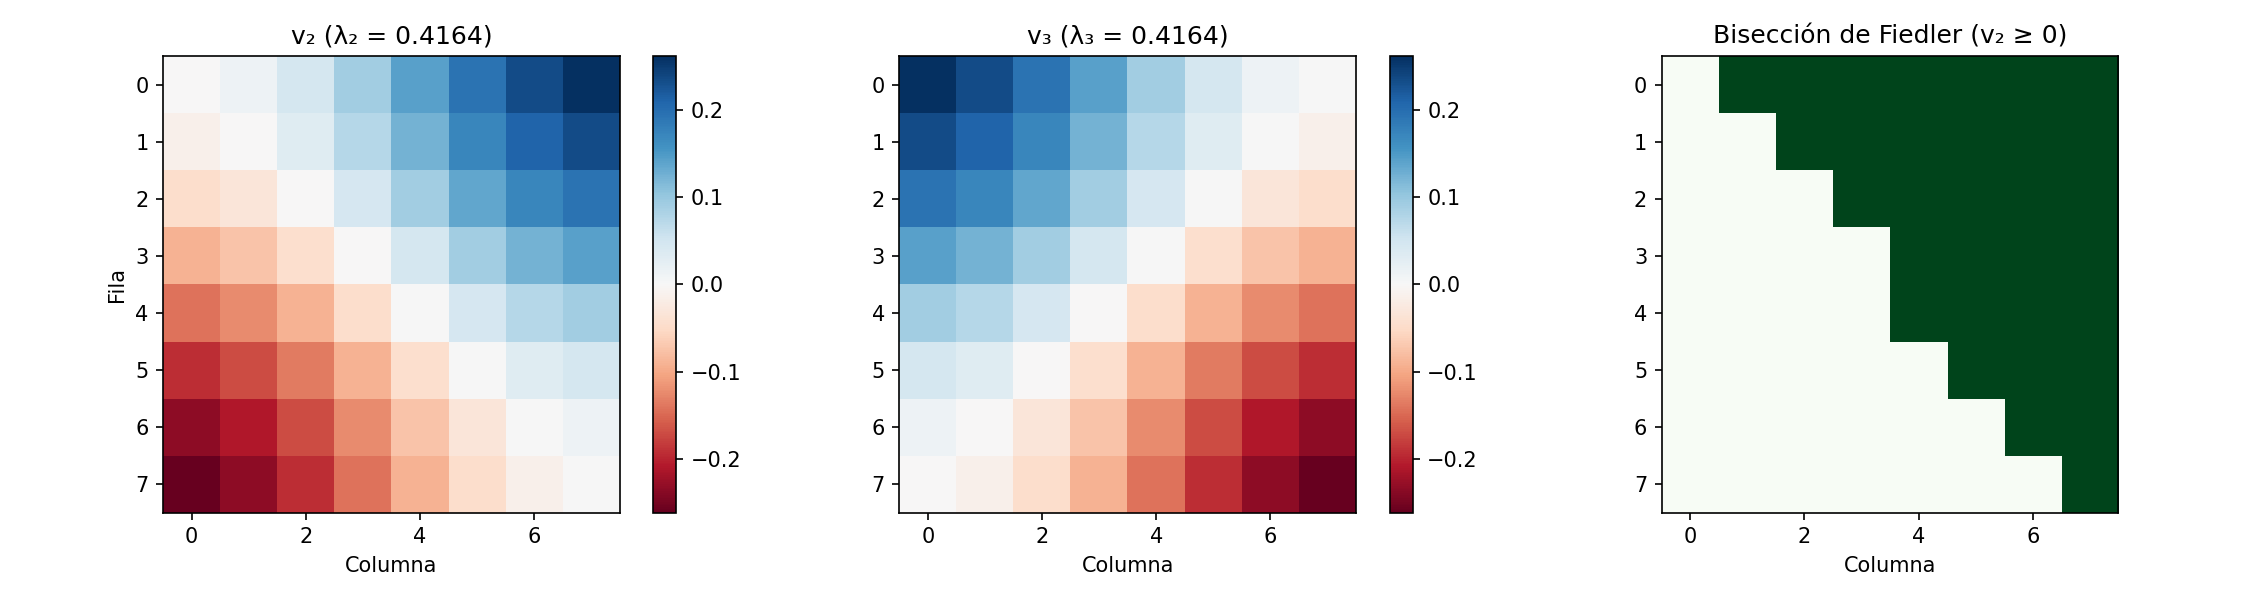
\includegraphics[width=\columnwidth]{../figures/fiedler_analysis.png}
    \caption{Análisis del eigenespacio de Fiedler en la grilla King $K(8,8)$. Se muestra la base diagonal (gradientes diagonales, corte de 28 aristas) versus la base axis-aligned (gradientes horizontal/vertical, corte óptimo de 22 aristas).}
    \label{fig:fiedler_eigenspace}
\end{figure}

\subsubsection{Optimalidad dentro del Eigenespacio}

\textbf{Proposición.} Para cualquier combinación lineal $\mathbf{u} = \alpha \mathbf{v}_2 + \beta \mathbf{v}_3 \in \mathcal{E}_2$ con $\alpha^2 + \beta^2 = 1$, la bisección $S_{\mathbf{u}} = \{v : u(v) \geq \text{mediana}(\mathbf{u})\}$ satisface:
\begin{equation}
    |E(S_{\mathbf{u}}, \bar{S}_{\mathbf{u}})| \geq 22
\end{equation}
con igualdad si y solo si $\mathbf{u}$ es proporcional a $\mathbf{w}_{\text{TB}}$ o $\mathbf{w}_{\text{LR}}$ (módulo perturbaciones angulares menores).

\textit{Demostración (verificación exhaustiva).} Parametrizando $\mathbf{u}(\theta) = \cos\theta \cdot \mathbf{v}_2 + \sin\theta \cdot \mathbf{v}_3$ con $\theta \in [0^\circ, 180^\circ)$, se evalúa computacionalmente el tamaño del corte para los 360 ángulos en incrementos de $0.5^\circ$. Los valores observados son $\{22, 24, 26, 28\}$, con mínimo $22$ alcanzado en $\theta \in [33^\circ, 57^\circ] \cup [123^\circ, 147^\circ]$, intervalos centrados en $\theta = 45^\circ$ y $\theta = 135^\circ$, que corresponden exactamente a $\mathbf{w}_{\text{TB}}$ y $\mathbf{w}_{\text{LR}}$. El máximo de $28$ se alcanza en $\theta = 0^\circ$ y $\theta = 90^\circ$ (los vectores diagonales originales). $\square$

\subsubsection{Implicación para la Comparación Humano--Algoritmo}

Este resultado tiene una consecuencia directa: el algoritmo estándar de bisección de Fiedler, al seleccionar un eigenvector arbitrario de $\mathcal{E}_2$, puede retornar un corte con $28$ aristas ($h = 28/210 = 0.1333$). En contraste, las díadas humanas que desarrollan divisiones Left-Right o Top-Bottom convergen a los cortes axis-aligned con $22$ aristas ($h = 22/210 = 0.1048$), que constituyen el \textbf{óptimo dentro del eigenespacio de Fiedler}.

El ratio de eficiencia espectral $\eta = h(S_{\text{Fiedler}})/h(S_{\text{obs}}) = 28/22 \approx 1.27$ no indica meramente que los humanos ``igualan'' al algoritmo, sino que lo \textbf{superan} al resolver implícitamente la ambigüedad del eigenespacio degenerado en favor de la dirección geométricamente óptima.

\subsection{Preguntas de Investigación}

\begin{enumerate}
    \item \textbf{Eficiencia espectral:} ¿Qué tan cerca está $h(S_{\text{obs}})$ de la cota inferior teórica $\lambda_2/2$?
    
    \item \textbf{Comparación con Fiedler:} ¿Es $h(S_{\text{obs}}) \approx h(S_{\text{Fiedler}})$? Es decir, ¿los humanos encuentran particiones comparables a la bisección espectral?
    
    \item \textbf{Tipos de división:} ¿Las divisiones Left-Right son más espectralmente eficientes que las divisiones Mixed?
    
    \item \textbf{Evolución temporal:} ¿Cómo evoluciona la eficiencia espectral a lo largo de las 60 rondas?
\end{enumerate}

% ============================================================================
% SECCIÓN 3: METODOLOGÍA PROPUESTA
% ============================================================================
\section{Metodología Propuesta}

\subsection{Pipeline de Análisis Espectral}

La metodología se centra en la comparación entre particiones observadas y particiones espectrales:

\subsubsection{Construcción del Laplaciano}

Para el grafo del tablero $G$:
\begin{itemize}
    \item Construir matriz de adyacencia $A$ (8-conectividad)
    \item Calcular matriz de grados $D$
    \item Obtener Laplaciano $L = D - A$
\end{itemize}

\subsubsection{Cálculo de Propiedades Espectrales}

\begin{itemize}
    \item Calcular eigenvalores y eigenvectores de $L$
    \item Extraer $\lambda_2$ (conectividad algebraica)
    \item Extraer $\mathbf{v}_2$ (vector de Fiedler)
    \item Obtener bisección espectral: $S_{\text{Fiedler}} = \{v : v_2(v) \geq 0\}$
\end{itemize}

\subsubsection{Extracción de Particiones Observadas}

Para cada díada $d$:
\begin{itemize}
    \item Calcular frecuencias de visita acumuladas por jugador
    \item Definir $S_{\text{obs}} = \{v : f_1(v) > f_2(v)\}$ (celdas dominadas por P1)
    \item Verificar conectividad de $S_{\text{obs}}$ mediante BFS (sanity check)
\end{itemize}

\subsubsection{Comparación de Conductancias}

Para cada díada, calcular y comparar:
\begin{itemize}
    \item $h(S_{\text{obs}})$: conductancia de la partición humana
    \item $h(S_{\text{Fiedler}})$: conductancia de la bisección espectral
    \item $\lambda_2/2$: cota inferior teórica (Cheeger lower bound)
\end{itemize}

\subsection{Algoritmo Principal}

\begin{algorithm}
\caption{Análisis de Eficiencia Espectral}
\begin{algorithmic}[1]
\REQUIRE Grafo $G$, Dataset SODCL
\STATE $L \leftarrow D - A$ \COMMENT{Matriz Laplaciana}
\STATE $\lambda_2, \mathbf{v}_2 \leftarrow$ Eigendecomposition($L$)
\STATE $S_{\text{Fiedler}} \leftarrow \{v : v_2(v) \geq 0\}$
\STATE $h_{\text{Fiedler}} \leftarrow$ Conductancia($S_{\text{Fiedler}}$)
\STATE $\text{cota} \leftarrow \lambda_2 / 2$
\FOR{cada díada $d$ en dataset}
    \STATE $S_{\text{obs}}^d \leftarrow$ ExtraerPartición($d$)
    \STATE $h_{\text{obs}}^d \leftarrow$ Conductancia($S_{\text{obs}}^d$)
    \STATE $\text{eficiencia}^d \leftarrow h_{\text{obs}}^d / h_{\text{Fiedler}}$
    \STATE $\text{gap}^d \leftarrow h_{\text{obs}}^d - \text{cota}$
\ENDFOR
\RETURN Distribución de eficiencias por tipo de división
\end{algorithmic}
\end{algorithm}

\subsection{Métricas de Evaluación}

\textbf{Ratio de Eficiencia Espectral:}
\begin{equation}
\eta_d = \frac{h(S_{\text{Fiedler}})}{h(S_{\text{obs}}^d)}
\end{equation}
Si $\eta_d \approx 1$, los humanos encuentran particiones comparables a la bisección espectral.

\textbf{Gap de Cheeger:}
\begin{equation}
\Delta_d = h(S_{\text{obs}}^d) - \frac{\lambda_2}{2}
\end{equation}
Mide qué tan lejos está la partición humana de la cota inferior teórica.

\subsection{Limitaciones y Riesgos}

El proyecto depende de: (1) parsing correcto del dataset SODCL y definición operativa de $S_{\text{obs}}$ mediante umbrales sobre frecuencias de visita; (2) interpretación adecuada de las particiones humanas en díadas con divisiones ambiguas (tipo ``mixed''). Por restricciones de tiempo, el análisis se centrará en un subconjunto de díadas con divisiones claras (Left-Right, Top-Bottom) y un grupo control de díadas ``mixed''. La evolución temporal se explorará como extensión si el pipeline principal funciona correctamente.

\textbf{Valores espectrales del grafo base (ya calculados):}
\begin{itemize}
    \item $\lambda_2 = 0.4164$ (conectividad algebraica)
    \item $h(S_{\text{Fiedler}}) = 0.1333$ (bisección espectral óptima)
    \item $|S_{\text{Fiedler}}| = 32$ (bisección balanceada)
\end{itemize}

% ============================================================================
% SECCIÓN 4: OBJETIVOS
% ============================================================================
\section{Objetivos}

\subsection{Objetivo General}

Determinar si las divisiones del trabajo emergentes en coordinación humana sin comunicación son \textbf{espectralmente eficientes}, comparando la conductancia de las particiones observadas con la bisección de Fiedler y la cota de Cheeger.

\subsection{Objetivos Específicos}

\begin{enumerate}
    \item \textbf{Modelar} el tablero experimental como grafo $G = (V, E)$ y construir su matriz Laplaciana $L$.
    
    \item \textbf{Calcular} el valor de Fiedler $\lambda_2$ y el vector de Fiedler $\mathbf{v}_2$, obteniendo la bisección espectral $S_{\text{Fiedler}}$.
    
    \item \textbf{Extraer} las particiones observadas $S_{\text{obs}}$ para cada díada basándose en frecuencias de visita acumuladas.
    
    \item \textbf{Comparar} la conductancia de particiones observadas $h(S_{\text{obs}})$ con la conductancia espectral $h(S_{\text{Fiedler}})$ y la cota inferior $\lambda_2/2$.
    
    \item \textbf{Analizar} si las divisiones Left-Right son más espectralmente eficientes que las divisiones Mixed o Top-Bottom.
    
    \item \textbf{Investigar} la evolución temporal de la eficiencia espectral a lo largo de las 60 rondas experimentales.
\end{enumerate}

% ============================================================================
% SECCIÓN 5: CRONOGRAMA
% ============================================================================
\section{Cronograma Tentativo}

\begin{tabular}{|l|l|l|}
\hline
\textbf{Semana} & \textbf{Actividad} & \textbf{Entregable} \\
\hline
1-4 & Modelado, Laplaciano, análisis exploratorio & Entrega 1 \\
5-8 & Cálculo de Fiedler y bisección espectral & Código v1 \\
9-11 & Extracción de particiones y conductancias & Entrega 2 \\
12-14 & Comparación Cheeger, análisis temporal & Código v2 \\
15-16 & Redacción final y presentación & Entrega 3 \\
\hline
\end{tabular}

% ============================================================================
% SECCIÓN 6: RESULTADOS ESPERADOS
% ============================================================================
\section{Resultados Esperados}

\textbf{Hipótesis principal:} Las díadas con divisiones claras (Left-Right, Top-Bottom) exhibirán $h(S_{\text{obs}}) \approx h(S_{\text{Fiedler}})$, indicando que los humanos convergen intuitivamente a particiones espectralmente óptimas.

\textbf{Hipótesis secundaria:} Las díadas con divisiones Mixed tendrán $h(S_{\text{obs}}) > h(S_{\text{Fiedler}})$, mostrando ineficiencia espectral.

\textbf{Implicación:} Si se confirma la hipótesis principal, sugeriría que la coordinación humana converge a particiones eficientes desde el punto de vista espectral.

% ============================================================================
% SECCIÓN 7: BIBLIOGRAFÍA
% ============================================================================
\bibliographystyle{IEEEtran}
\begin{thebibliography}{10}

\bibitem{andrade2021}
E. Andrade-Lotero and R. L. Goldstone, ``Self-organized division of cognitive labor,'' \textit{PLOS ONE}, vol. 16, no. 7, p. e0254532, Jul. 2021.

\bibitem{chung1997}
F. R. K. Chung, \textit{Spectral Graph Theory}. Providence, RI: American Mathematical Society, 1997.

\bibitem{fiedler1973}
M. Fiedler, ``Algebraic connectivity of graphs,'' \textit{Czechoslovak Mathematical Journal}, vol. 23, no. 2, pp. 298--305, 1973.

\bibitem{mesbahi2010}
M. Mesbahi and M. Egerstedt, \textit{Graph Theoretic Methods in Multiagent Networks}. Princeton, NJ: Princeton University Press, 2010.

\bibitem{vonluxburg2007}
U. von Luxburg, ``A tutorial on spectral clustering,'' \textit{Statistics and Computing}, vol. 17, no. 4, pp. 395--416, Dec. 2007.

\bibitem{cheeger1970}
J. Cheeger, ``A lower bound for the smallest eigenvalue of the Laplacian,'' in \textit{Problems in Analysis}, Princeton, NJ: Princeton University Press, 1970, pp. 195--199.

\bibitem{mohar1991}
B. Mohar, ``The Laplacian spectrum of graphs,'' in \textit{Graph Theory, Combinatorics, and Applications}, vol. 2, Y. Alavi et al., Eds. New York: Wiley, 1991, pp. 871--898.

\bibitem{newman2018}
M. Newman, \textit{Networks}, 2nd ed. Oxford: Oxford University Press, 2018.

\bibitem{goldstone2024}
R. L. Goldstone, E. Andrade-Lotero, R. D. Hawkins, and M. E. Roberts, ``The emergence of specialized roles within groups,'' \textit{Topics in Cognitive Science}, 2024.

\end{thebibliography}

\end{document}
